\chapter{Desenvolvimento do tema}
\label{cap:experiments}

Este capítulo é opcional e, a existir, é aqui que deve descrever como é que o seu projecto evoluiu.

O projeto é constituido em seis partes:

\begin{enumerate}
    \item Ambiente de teste do projeto;
    \item Testes de Firewall e conexões realizados;
    \item Testes da API do LXD;
    \item \textit{"Port Controller"} - daemon em C\#;
    \item API e Interface Web;
    \item Sitema de notificações;
\end{enumerate}


No final o ambiente do projeto será o da seguinte imagem:

\begin{figure}[H]
\begin{center}
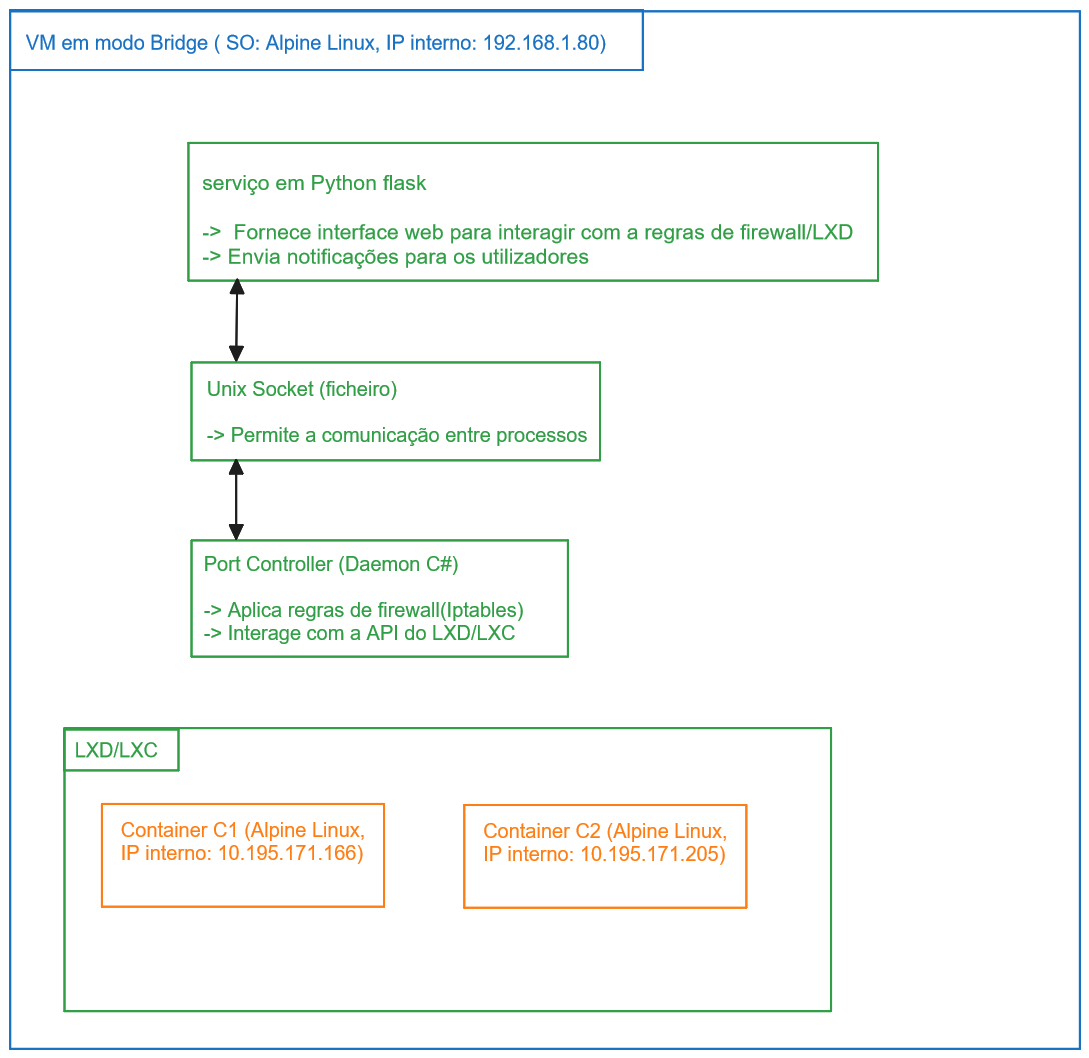
\includegraphics[width=14cm]{figs/estrutura2.png}
\caption{Abiente do projeto}
\label{fig:bookstack}
\end{center}
\end{figure}



\section{Ambiente de testes do projeto}

Esta secção do relatório irá abordar os passos efetuados na configuração do sistema 
usado como ambiente de testes do projeto e respetivas aplicações/pacotes instalados.

Sendo os seguintes:
\begin{enumerate}
    \item Configuração do Alpine Linux;
    \item Configuração do LXD/LXC;
    \item Instalação do .NET Core;
    \item Instalação de outros pacotes;
\end{enumerate}


\subsection{Configuração do Alpine Linux}

De modo a obter, os melhores resultados possiveis durate os estes e experiencias
ao longo deste projeto é de extrema importância que o sistema operativo de testes
seja o mesmo da plataforma Forge. Sendo assim foi intalada numa máquina virtual
VMware com o alpine linux 3.19.

Especificações atribuidas à maquina virtual:

\begin{itemize}
    \item 6 GB de RAM;
    \item 3 nucleos de para o CPU;
    \item Placa de rede no modo Bridge;
    \item 40 GB de armazenamento;
\end{itemize}

De seguida foi feita a configuração inicial do sistema com os seguintes coamandos:


\begin{enumerate}
    \item \texttt{localhost login: root 
    \item setup-alpine
    \item Select keyboard layout: pt-pt
    \item Enter a system hostname : alpine
    \item Which one do you want to initialize? [eth0]
    \item Ip address for eth0? [dhcp]
    \item Do you want to do any manual network configuration? (y/n) [n] n
    \item (Changing password for root) New password: ******
    \item which timezone are you in [UTC]
    \item HTTP/FTP proxy URL? [none]
    \item Enter mirror number (1-72) or URL to add (or r/f/e/done) [1]
    \item Setup user? (enter a lower-case loginname, or 'no') [no] delta
    \item Password: ******}
    \item Enter ssh key or URL for titus (or 'none') [none]
    \item Which ssh server ('openssh', 'dropbear', or 'none') [openssh]
    \item Which disk(s) would you like to use? [none] sda 
    \item how you would like to use it? ('sys', 'data', 'crypt', 'lvm' or '?'for help) [?] sys 
    \item Erase the above disk(s) and continue? (y/n) [n] y 
    \item Instalation Complete. Please reboot.
\end{enumerate}


\textbf{Nota:} As opcções \textit{default} são sugeridas dentro de "[]" caso se pretenda
usar essa opção é apenas necessário carregar na tecla "\textit{ENTER}". \\


Para terminar a configuração foi executado o comando: 

%\texttt{apk add --upgrade apk-tools \&\& apk upgrade --available} \\

\begin{tcolorbox}[colback=blue!5!white,colframe=blue!75!black]
    \verb |doas apk add --upgrade apk-tools \&\& apk upgrade --available |
\end{tcolorbox}

Foi também ativado o repositório da comunidae para ter um maior
numero de pacotes para instalar. Para isto é necessário descomentar a linha no
ficheiro "\textit{repositories}" com a localização "/etc/apk/repositories" com o
URL deste repositório, removendo o "\#" no inicio da linha.

No final o conteúdo do ficheiro deverá ser este:

\begin{lstlisting}[language=Bash, caption={Ficheiro repositories}]
http://dl-cdn.alpinelinux.org/alpine/v3.19/main
http://dl-cdn.alpinelinux.org/alpine/v3.19/community
\end{lstlisting}

\subsection{Configuração do LXD/LXC}

No que diz respeito ao LXD/LXC foram instalados os pacotes lxd e lxd-client.


Foi ativado o serviço do lxd como default com o comando \texttt{rc-update add lxd default}
e em seguida ativado com o \texttt{rc-service lxd start}.

Depois foi feita a configuração iniciul com o comando texttt{lxd init} com a seguintes opções:

\begin{enumerate}
    \item \texttt{Would you like to use LXD clustering? (yes/no) [default=no]: no
    \item Do you want to configure a new storage pool? (yes/no) [default=yes]: yes
    \item Name of the new storage pool [default=default]: default
    \item Name of the storage backend to use (btrfs, dir, lvm, zfs) [default=zfs]: dir
    \item Would you like to connect to a MAAS server? (yes/no) [default=no]: no;
    \item Would you like to create a new local network bridge? (yes/no) [default=yes]: yes
    \item What should the new bridge be called? [default=lxdbr0]: lxdbr0
    \item What IPv4 address should be used? (CIDR subnet notation, “auto” or “none”) [default=auto]: auto
    \item What IPv6 address should be used? (CIDR subnet notation, “auto” or “none”) [default=auto]: auto
    \item Would you like LXD to be available over the network? (yes/no) [default=no]: no
    \item Would you like stale cached images to be updated automatically? (yes/no) [default=yes] yes
    \item Would you like a YAML "lxd init" preseed to be printed? (yes/no) [default=no]: no}
\end{enumerate}

De seguida foi editada a configuração \textit{default} com o 
comando "\texttt{lxc profile edit default}" nela deverá ser garantida o
seguinte:

\begin{lstlisting}[language=csh, caption={edição do perfil padrão}]
  eth0:
    name: eth0
    nictype: bridged
    parent: lxdbr0
    type:nic

\end{lstlisting}

\textbf{Nota:} eth0 é a interface do sistema \textit{host} e lxdbr0 é a interface
de rede criada automaticamente pelo LXD.

Com esta configuração os \textit{containers} irão funcionar em modo NAT.


Após isto foram criados dois containers Alpine linux com o seguinte 
comando: % "\texttt{lxc launch images:alpine/3.19 <nome do container>}"

\begin{tcolorbox}[colback=blue!5!white,colframe=blue!75!black]
    \verb |doas lxc launch images:alpine/3.19 <nome do container> |
\end{tcolorbox}

Podendo assim serem listados com o comando:

\begin{tcolorbox}[colback=blue!5!white,colframe=blue!75!black]
    \verb |doas lxc list |
\end{tcolorbox}


A seguinte imagem mostra o output do comando acima referido.

\begin{figure}[H]
\begin{center}
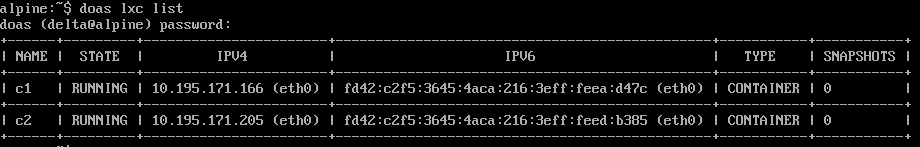
\includegraphics[width=14cm]{figs/lista de containers.png}
\caption{Containers criados.}
\label{fig:bookstack}
\end{center}
\end{figure}



\subsection{Instalação do .NET Core}


Para depois poder executar a aplicação que irá controlar as portas dos containers,
aplicação esta desenvolvida em C\# .NET Core é necessário instalar os pacotes necessários
para o funcionamento da mesma, mais concretamente o sdk e o \textit{runtime}.

Os pacotes necessŕios foram instalados usando os seguintes comandos:
\begin{itemize}
    \item \texttt{doas apk add dotnet7-sdk};
    \item \texttt{doas apk add dotnet7-runtime};
\end{itemize}




\subsection{Instalação de outros pacotes}

Para além do .NET Core, para garantir o funcionamento das aplicações desenvolvidas neste projeto é necessário
instalar ainda os seguintes pagotes:
\begin{itemize}
    \item Python - \texttt{doas apk add python3};
    \item Pip - \texttt{doas apk add python3-pip}
    \item Bash - \texttt{doas apk add bash};
\end{itemize}


Para uma maior facilidade de uso do sistema durante o seu uso foi também instalado
o "tmux" que permite criar "janelas" e trocar rapidamente entre as mesma, funcionalidade
essa que aumenta a produtividade num ambiente de apenas terminal.
Para asua instala ção foi usado o comando:
\begin{itemize}
    \item \texttt{doas apk add tmux};
\end{itemize}







%==========================================================================


\section{Testes de Firewall e conexões realizados}

Uma vez os \textit estarem configurados em modo NAT seria necessário criar regras 
de redirecionamento de portas ou endereços IP de modo a os \textit{containers} serem acedidos
por outros dispositivos na rede local.


De modo a realizar testes de conexão foram instalados dentro dos containers
o netcat e o python.

\textbf{Nota:} eth0 é a placa de rede do sistema host e tem o ip local de 192.168.1.80.


Durante os testes realizados, concluiu-se que existem três medodos de criar conectividade:

\subsection{Método 1: Criar regras no lxc network e defenir portas de redirecionamento}

\textbf{Nota:} Neste metodo será usado como exemplo o \textit{container} "c2" que
dentro da máquina virtual host tem o IP 10.195.171.166.

\textbf{Nota nº2:} A máquina virtual \textit{Host} tem o endereço IP 192.168.1.80.

Este metodo usa o comando "\texttt{lxc network forward create lxdbr0 192.168.1.80}"
para criar a regra e "\texttt{lxc network forward port add lxdbr0 192.168.1.80 tcp 7000 10.195.171.205 8000}"
para adicionar as portas a serem reencaminhadas, neste exemplo o trafego vindo da
rede local que tenta aceder ao endereço IP 192.168.1.80 (\textit{host}) pela porta 7000 será redirecionado
para a porta 8000 do IP 10.195.171.205 que pertence ao container "c2".

Nesta experiência o container está a executar um servidor http na porta 8000
com o comando "\texttt{python3 -m http.server}".


\textbf{Nota:} Porta 8000 é a padrão quando não é especificada outra no final do comando.


Foi possivel aceder ao servidor HTTP pelo browser num computador da rede local.

\begin{figure}[H]
\begin{center}
\includegraphics[width=12cm]{figs/teste de conexão via browser.png}
\caption{Teste de conexão via browser.}
\label{fig:bookstack}
\end{center}
\end{figure}


Foram também usados alguns comandos do netcat como o seguinte: % "\texttt{nc -w1 -vz 192.168.1.80 7000}".

\begin{tcolorbox}[colback=blue!5!white,colframe=blue!75!black]
    \verb | nc -w1 -vz 192.168.1.80 7000 |
\end{tcolorbox} 


\begin{figure}[ht]
\begin{center}
\includegraphics[width=12cm]{figs/teste de conexão1.png}
\caption{Teste de conexão com o netcat.}
\label{fig:bookstack}
\end{center}
\end{figure}

Foram usados também usados os comandos "\texttt{nc 192.168.1.80 7000} e \texttt{nc -l 8000}"
de modo a criar uma ligação TCP. Foi também testado a ligação reversa
onde o \textit{container} se tenta ligar ao computador da rede, invertendo os comandos
"\texttt{nc 192.168.1.68 3000}" e "\texttt{nc -l 3000}", ambos os testes foram bem
sucedidos.







\subsection{Método 2: Usar um IP para redirecionar o tráfego para o container}

Neste método é atribuido um endereço ip da rede local, que esteja disponivel, à
interface de rede do sistema host, eth0, usado o comando
"\texttt{ip address add 192.168.1.120/24 dev eth0}", para este exemplo foi escolhido o IP
"192.168.1.120".

De seguida, é necessário criar a regra de redirecionamento do tráfego
com o IP de destino "192.168.1.120" para o IP de um \textit{container}, que neste esxemplo será o
IP "10.195.171.166" que pertence ao \textit{container} "c1", para isto foi usado o
comando "\texttt{lxc network forward create lxdbr0 192.168.1.120 target\_address=10.195.171.166}"
que automaticamente cria uma regra na tabela NAT do iptables para garantir o correto
funcionamento do redirecionamento.

Com esta configuração se o \textit{container} "c1" que possui o IP "10.195.171.166" estiver a executar um servidor 
http na porta 8000, o mesmo serviço estará disponivel para dispositivos da rede local
através do IP 192.168.1.120 na porta 8000.

\textbf{Nota:} Os testes de conexão usados no método 1 foram igualmente bem sucedidos.


Após usar o comando "\texttt{lxc network create <network name> <listen address>}", é ainda possivel pecificar portas com o seguinte comando:

\begin{tcolorbox}[colback=blue!5!white,colframe=blue!75!black]
    lxc network forward port add $<$network\_name$>$ $<$listen\_address$>$ $<$protocol$>$ $<$listen\_ports$>$ $<$target\_address$>$ $[<$target\_ports$>]$
\end{tcolorbox}

O seguinte exemplo mostra a associação do IP do \textit{container} da porta 22 com a porta 22 do IP externo atribuído (192.168.1.120).

\begin{tcolorbox}[colback=blue!5!white,colframe=blue!75!black]
    lxc network forward port add lxdbr0 192.168.1.120 tcp 22 10.195.171.166 22
\end{tcolorbox}

\subsection{Método 3: Usar o Iptables para criar portas de redirecionamento}

O método 3 é o mesmo que o médotos anteriores mas só que configurado usando apenas regras
do Iptables, ou seja, é criaca uma regra na tablea NAT que redireciona o tráfego
de uma porta do sistema host para um IP e porta de um \textit{container}.

É possivel criar esta configuração com o comando:



%\begin{lstlisting}[language=Bash, caption={Exemplo de regra de redirecionamento}]
%    doas iptables -t nat -I PREROUTING -p tcp --dport 5000 -j DNAT --to-destination 10.195.171.205:8000
%\end{lstlisting}

\begin{tcolorbox}[colback=blue!5!white,colframe=blue!75!black]
    doas iptables -t nat -I PREROUTING -p tcp --dport 5000 -j DNAT --to-destination 10.195.171.205:8000
\end{tcolorbox}

Neste exemplo similar ao exemplo do método 1, se o \textit{container} "c2" com o 
endereço IP "10.195.171.205", estiver a executar um servidor HTTP na porta
8000, os dispositivos na rede local poderão aceder a este serviço acedendo à porta 
5000 do IP do sistema host(192.168.1.80).


Da mesma forma que o método 2 è possivel associar também um IP externo com o seguinte comando de exemplo
onde é feita a associação da porta 22 juntamente com o ip externo atribuído:

Importante referir, que antes deste de criar a regra no iptables é necessário usar o
comando ”\texttt{ip address add 192.168.1.120/24 dev eth0}”, para adicionar o endereço IP
à placa de rede do sistema.

\begin{tcolorbox}[colback=blue!5!white,colframe=blue!75!black]
    doas iptables -t nat -I PREROUTING -p tcp --dport 22 -d 192.168.1.120 -j DNAT --to-destination 10.195.171.166:22
\end{tcolorbox}



\textbf{Nota:} Os testes de conexão usados no método 1/2 foram igualmente bem sucedidos.




% =============================================================================
% =============================================================================



\section{Testes da API do LXD}


Após os testes referidos na secção anterior, terem sido concluídos, foi necessário
reproduzir os mesmos resultados, mas com a API do LXD.

A vantagem principal em usar este método está na performance da interação do "Port Controller" com
o LXC, que no momento de criar uma regra, será criado menos um processo, do que 
usar o "Port Controller" para executar um comando do LXC/LXD na \textit{shell} do sistema.

Portanto, após consultar a \href{https://documentation.ubuntu.com/lxd/en/latest/api/#/}{documentação oficial da API do LXD},
nomeadamente, a secção "network-forwards" foram realizados com sucesso, auxilio do comando curl, os seguintes testes:


Importante referir que para um melhor funciuonamento da API e de modo a evitar erros,
é recomendado os endereços IP, que se prentendam atribuir a um \textit{container} 
sejam previamente adicionados e associados ao "LXC forward" com um dos seguintes comandos:

\begin{tcolorbox}[colback=blue!5!white,colframe=blue!75!black]
    lxc network forward create $<$network\_name$>$ $<$listen\_address$>$
\end{tcolorbox}

\begin{tcolorbox}[colback=blue!5!white,colframe=blue!75!black]
    lxc network forward create lxdbr0 192.168.1.120
\end{tcolorbox}


ou com o curl e com o IP "192.168.1.120" a servir de IP externo:


\begin{lstlisting}[language=Bash, caption={Exemplo para registar um IP para redirecionar trafego (API do LXD)}]
    curl --unix-socket /var/lib/lxd/unix.socket -X POST -d '{"config":{},"description":"","listen_address":"192.168.1.120","ports":[]}'  lxd/1.0/networks/lxdbr0/forwards
\end{lstlisting}


Após isso, exclusicamente através da API do LXD é necessário associar o IP externo previamente
adicionado com o endereço IP do \textit{container} e respetivas portas.

É possivel realizar esta operação com uma solicitação "PUT" para a API do LXD

\begin{lstlisting}[language=Bash, caption={Exemplo de associação de IPs e portas usando a API do LXD}]
    curl --unix-socket /var/lib/lxd/unix.socket -X PUT -d '{"config":{},"description":"10.195.171.166","listen_address":"192.168.1.120","ports":[{"description":"","listen_port":"7000","protocol":"tcp","target_address":"","target_port":"8000"}]}'  lxd/1.0/networks/lxdbr0/forwards/192.168.120
\end{lstlisting}


No exemplo acima é criada a associação entre a potra 8000 do IP "10.195.171.166" que pertence a 
um \textit{container} e a porta 7000 do IP externo "192.168..1.120".

Uma fez realizado com sucesso este teste será apenas necessário implementar esta 
mesma solicitação no "Port Controller". \\






\textbf{Nota:} Caso se pretenda criar conexão exclusivamente através de IPs sem especificar portas é 
possivel, no momento de adição do IP externo ao "LXD forward" usar a seguinte comando:

\begin{lstlisting}[language=Bash, caption={Exemplo para registar um IP e associá-lo a um cinatiner (API do LXD)}]
    curl --unix-socket /var/lib/lxd/unix.socket -X POST -d '{"config":{"target_address":"10.195.171.166"},"description":"","listen_address":"192.168.1.120","ports":[]}'  lxd/1.0/networks/lxdbr0/forwards
\end{lstlisting}

Esta solicitação efetuada com o curl tem o mesmo resultado do comando:

\begin{tcolorbox}[colback=blue!5!white,colframe=blue!75!black]
   lxc network forward create lxdbr0 192.168.1.120 target\_address=10.195.171.166
\end{tcolorbox}








% =============================================================================
% =============================================================================


\section{Criação da API}

Para interagir com o daemon C\# (Port Controller) responsável por interagir com regras do iptables
e configurações do LXC/LXD, foi criada uma API em Python com a biblioteca Flask como
método alternativo à interface \textit{Web}.

O principal motivo da criação desta API é a facilitação nos momentos de teste dos programas
desenvolvidos, uma vez que pode ser testada no terminal com o comando Curl. Contudo, nada 
impede o administrador do sistema de usar este método de interação com o "Port Controler"
como forma principal, uma vez que funciona de formna independente da interface Web.

Sendo assim, neste componente do projeto desenvolvida em Python à três partes essênciais:

\begin{enumerate}
    \item API - que permite ao utilizador (administrador do sistema) interagir com o "Port Controller" daemon em C\#
    através do terminal fazendo solicitações HTTP com o comando Curl;
    \item Interface Web - que permite ao utilizador (administrador do sistema) interagir com o "Port Controller"
    através de uma interface gráfica que pode ser acedida através do \textit{browser};
    \item O ficheiro (unixSocketConn.py) que comunica com a unix socket (localizada em /tmp/socket\_proj) que por sua vez, comunica com o "Port Controller". 
\end{enumerate}

Nesta secção o foco será a explicação do funcionamento da API, porém, para esclarecer
melhor o funcionamentodos ficheiros referidos a seguinte imagem
mostra o fluxo de comunicação entre os ficheiros/programas do projeto.

\begin{figure}[H]
\begin{center}
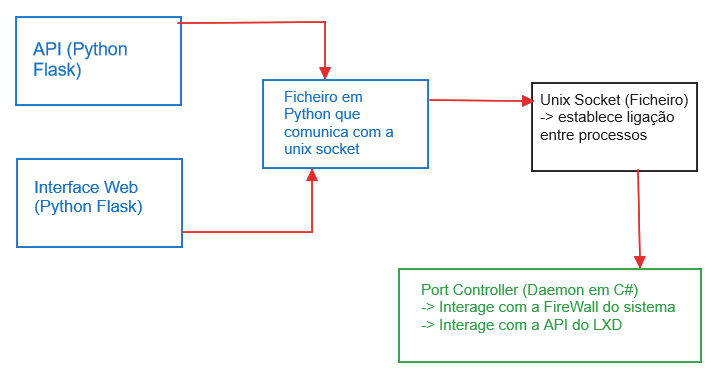
\includegraphics[width=14cm]{figs/fluxo de comunicação.png}
\caption{Fluxo de comunicação do projeto}
\label{fig:bookstack}
\end{center}
\end{figure}



\subsection{Pré-requesitos}

Uma vez que esta componte de API de projeto é feita usando a linguagem Python é necessário
usar as seguintes bibliotecas:

\begin{itemize}
    \item Flask - biblioteca responsável pela criação da API;
    \item re - biblioteca usada para expressões regulares;
    \item json - biblioteca para manipulação de contúdo em fm formato JSON;
\end{itemize}
    
Das bibliotecas mencionadas apenas o "Flask" é externa, sendo necessário instalar a mesma
com o seguinte comando:

\begin{tcolorbox}[colback=blue!5!white,colframe=blue!75!black]
    \verb | doas apk add py-flask |
\end{tcolorbox}

\textbf{Nota:} O Alpine linux não permite instalar bibliotecas/pacotes usando o "pip" (gestor de pacotes
do python) de forma direta.

Após intalado é necessário garantir as seguintes linhas no ficheiro "main" da API.

\begin{lstlisting}[language=csh, caption={Importações necessárias}]
from flask import Flask, request, jsonify
import re
import json
from unixSocketConn import *
\end{lstlisting}

A linha 4 é faz importação das funções defenidas do ficheiro "unixSocketConn.py", ficheiro esse, 
responsável for enviar dados para o ficheiro da unxix socket.


\subsection{Estrutura da API}

A API está dividida em três partes/caminhos URL:

\begin{enumerate}
    \item  \slash host\_fw - onde as solicitações feitas para este URL serão relacionadas à interação
    com a Firewall do sistema, mais concretamnte a tabela Filter do Iptables\slash Nftables;
    \item  \slash host\_nat - neste caminho as solicitações são relacionadas à interação com
    com a Firewall do sistema mas direcionadas à tabela NAT ou regras do LXD Forward;
    \item  \slash cont\_port (caminho secundário/opcional) - Neste caminho as solicitações, têm o objetivo de interagir com regras de firewall
    (Iptables ou nftables) dentro de \textit{containers} alojados dendoro do sistema \textit{host}. 
\end{enumerate}


\title*{\textbf{Exemplo de código}}

No seguinte excerto de código mostra um a implementação de um caminho da API (\slash host\_nat)

\begin{lstlisting}[language=Bash, caption={Definição de um caminho}]
@app.route("/host_fw", methods=["POST"]) # executar no host
def host_fw():
    
    try:

        data = request.get_json()
        
        action = data['Action']
        firewall = data['Fw']
        protocol = data['Protocol']
        porta = data['Port']

    except:
        print("Erro ao receber dados!")
        return "Error ao receber os dados", 500
    else:

        hostfw(action, firewall, protocol, porta)
        
        return jsonify(data, "Solicitacao bem sucedida!"), 201  
\end{lstlisting}

Neste excerto de código está a função responsável por receber a solicitação \textit{POST}.
Dentro da secção do "try" os valores enviados em JSON pela solicitação serão guardados em
variáveis para depois serem passados para a função "hostfw" função essa que percente ao ficheiro
"unixSocketConn.py". As funções presentes neste ficheiro após receberem os valores vindos 
da solicitação enviam os dados formatados em JSON para o ficheiro da unix socket (/tmp/socket\_proj) que por sua vez,
chegará ao "Port controller".



\subsection{Definição dos parâmetros}

Para fazer uma solicitação para um destes caminho foram defenidos parâmetros\slash argumentos
que podem ser enviados, os mesmos podem visualizados na seguinte tabela:

\begin{table}[H]
\centering
\begin{tabular}{|c|c|}
\hline
\rowcolor{yellow!50}\textbf{Parâmetros} & \textbf{Opções}\\
\hline
Container & $<$Container name$>$\\
\hline
Type & lxc, incus \\
\hline
Action & ClosePort, OpenPort, AddNat, RemoveNat, ResetNat, ExecCmd \\
\hline
Fw & ipt, nft, lxcforward, lxdapi \\
\hline
Port & $<$numero entre 1-65535$>$ \\
\hline
protocol & tcp, udp \\
\hline
Container\_internal\_ip & $<IP>$ \\
\hline
Container\_internal\_port & $<$numero entre 1-65535$>$ \\
\hline
Rule & $<$Regra costumizada e opcional para usar na Firewall(Iptables ou Nftables)$>$ \\
\hline
\end{tabular}
\caption{Lista de parâmetros possiveis de usar.}
\label{arglist}
\end{table}

\textbf{Nota:} Os parâmetros não são todos obrigatórios, alguns dependem do URl para o qual
se pretende fazer solicitação.


\subsection{Formato da solicitação}

Para fazer uma solicitação para um URL da API será usado o comando curl como exemplo para
cada um dos caminhos criados.

As solicitações devem ser feitas deve ser do tipo POST de modo a enviar dados com os parãmetros
corretos para aquele aquele caminho e em formato JSON.

Com comando "curl" é especificado o tipo de solicitação com a "flag" \texttt{-X <tipo de solicitação>},
o cabeçalho com a flag \texttt{-H "<Conteúdo do cabeçalho>"}, de seguida com a flag -d os parâmetros
em formato JSON dentro de aspas simples e por fim, o URL completo para o qual se prentende enviar a
solicitação.



\title*{Exemplo para \slash \textbf{host\_fw}}

\begin{lstlisting}[language=Bash, caption={Exemplo de solicitação para a firewal do sistema host}]
    curl -X POST -H "Content-Type:application/json" -d '{"Action":"OpenPort","Fw":"ipt","Protocol":"tcp","Port":"22"}' http://localhost:5000/host_fw
\end{lstlisting}



Como se pode observar neste exemplo para o caminho "host\_fw" os parâmetros passados devem ser:

\begin{enumerate}
    \item Action;
    \item Fw;
    \item protocol;
    \item Port;
    \item Rule (Opcional);
\end{enumerate}

Opcionalmente é possivel usar o parâmetro "Rule" e especificar uma regra para o Iptables\slash Nnftables
para tal o parâmetro "\textit{Action}" deve ser "ExecCmd", o parâmetro "Fw" deve ser referido normalmente com "ipt" ou "nft" e os restantes devem ser mencionados mas vazios, como no seguinte exemplo:

\begin{lstlisting}[language=Bash, caption={Exemplo de solicitação para a firewal do sistema host com uma regra personalizada}]
    curl -X POST -H "Content-Type:application/json" -d '{"Action":"ExecCmd","Fw":"ipt","Protocol":"","Port":"", "Rule":"INPUT -s 192.168.1.140 -j DROP"}' http://localhost:5000/host_fw
\end{lstlisting}



\title*{\textbf{host\_nat}}

\begin{lstlisting}[language=Bash, caption={Exemplo de solicitação para a firewal do sistema host para associar um IP externo a umIp de container de modo a criar conectividade}]
    curl -X POST -H "Content-Type:application/json" -d '{"Action":"AddNat","Fw":"ipt","Protocol":"tcp","Port":"22","External_ip":"192.168.1.120","Container_internal_ip":"10.195.171.205","Container_internal_port":"80" }' http://localhost:5000/host_nat
\end{lstlisting}

Neste exemplo pretende-se criar conectividade criando uma regra na tabela NAT do iptables de modo a associar
um IP interno de um \textit{container} com um IP externo escolhido pelo administrador do sistema.

É possivel executar o comando comando de igual forma trocando apenas o parâmetro "Fw" para "lxdforward" 
ou "lxdapi" de modo a criar a mesma associação mas através do LXD, tanto um como outro criará uma regra
semelhante ao Iptables de forma automática.

A vantagem principal está em usar a opção "lxdapi", que como nome indica irá usar a API do LXD para
criar a regra, que em comparação com as outras opções garante performance extra uma vez que não é necessária
a criação de um novo processo para criar uma regra. De qualquer forma este tópico será abordado e explicado mais detalhadamente 
na secção de explicação do "Port Controller". \\


\title*{\textbf{cont\_port}}

\begin{lstlisting}[language=Bash, caption={Exemplo de solicitação para a firewal do sistema host para associar um IP externo a umIp de container de modo a criar conectividade}]
    curl -X POST -H "Content-Type: application/json" -d '{"Container":"c1","Type":"lxc","Action":"OpenPort","Fw":"ipt", "Protocol":"tcp","Port":"22"}' http://localhost:5000/cont_port
\end{lstlisting}

Com uma estrutura similar à solicitação feita para o "host\_fw", as solicitações para o caminho "cont\_port"
devem apenas incluir os parâmetros "Container" e "Type".
\begin{enumerate}
    \item Container;
    \item Type;
    \item Action;
    \item Fw;
    \item protocol;
    \item Port;
    \item Rule (Opcional);
\end{enumerate}




\subsection{ligação à unix socket}

O seguinte excerto de código mostra como funciona uma função no ficheiro "unixSocketConn.py" responsável
para se ligar à unix socket, localizada em "/tmp/socket\_proj" (localização da unix socket
é opcional) e assim enviar os dados atrvés da mesma para o "Port Controller".

\begin{lstlisting}[language=Bash, caption={Definição de um caminho}]
def hostfw(action, firewall, protocol, porta):

socket_path = socketPath()

try:
    # Criar uma Unix socket
    client_socket = socket.socket(socket.AF_UNIX, socket.SOCK_STREAM)

    # Conectar a Unix socket
    client_socket.connect(socket_path)

    # Enviar uma mensagem para o servidor
    
    json_data = {
        "Type": "host",
        "Action": action,
        "Fw": firewall,
        "Protocol": protocol,
        "Port": porta
    }
    
    client_socket.send(json.dumps(json_data).encode())


    time.sleep(1.5)
    # Receber a resposta 
    response_json = client_socket.recv(1024).decode()
    response = json.loads(response_json)

    # mostrar a resposta
    print("Status:", response["Status"])
    print("Mensagem:", response["Mensagem"])

    # Fechar o socket
    client_socket.close()

except Exception as e:
    print("Ocorreu um erro:", e)  
\end{lstlisting}


É possivel observar la linha 7 a definição do tipo se socket e o tipo de transferênia,
na linha 14 é defenida a estrura em JSON que será envida, nela o paraaâmetro "Type" é 
defenida como "host" de modo a informar o "Port Controller" que é o alvo do comando/regra a ser
executado é o próprio sistema \textit{host}.

De seguida, na linha 22 a estrutura json é formatada e envida para a unix socket.

O código seguinte é responsável por receber a resposta do "Port Controller", por fim, a conexão
é com a unix socket é fechada na linha 35. 










% =============================================================================

\section{Port Controller}

\subsection{Escolha da tecnologia}

Uma vez que a plataforma forge funciona no sistema \textit{Alpine Linux} seria
necessário escolher ferramentas suportadas por esta distribuição.

No caso desta parte do projeto, foi escolhida a linguagem C\# com o 
\textit{framework} .NET Core versão 7.0.



\subsection{Funcionalidades}

"Em sistemas operativos de computador multitarefa, um daemon é um programa de 
computador executado como um processo em segundo plano, em vez de estar sob o 
controle direto de um utilizador interativo. Tradicionalmente, os nomes dos processos
de um daemon terminam com a letra d, para esclarecer que o processo é de fato um 
daemon e para diferenciar entre um daemon e um programa de computador normal." \cite{daemon}

Este componente do projeto, denominado de "Port Controller", tem como objetivo,
funcionar constantemente em segundo plano, para controlar as conexões ao
sistema\textit{host} e dos \textit{containers} nele alojados.

O \textit{"Port Controller"} tem como principal função estar à escuta de pedidos
do administrador e executar estes pedidos na \textit{Firewall} do sistema
\textit{host} (Iptables) ou a API do LXD de modo a gerir conexões relacionadas 
com os \textit{containers} ativos ou ao próprio sistema \textit{host}.
Os pedidos são recebidos na componente da \textit{unix socket} em formato
\textit{JSON}.


Opcionalmente, o \textit{"Port Controller"} é também capaz de interagir com \textit{containers}
do tipo LXC e executar comandos dentro destes para interagir com a
\textit{Firewall} Iptables ou Nftables.

\subsection{Estrutura do código}

O código do "Port Controller" é constituido pelos seguintes ficheiros:

\begin{itemize}
    \item Program.cs;
    \item SocketData.cs;
    \item Firewall.cs
    \item Container.cs
    \item Lxc.cs

\end{itemize}


\subsection{Funcionamento do código}

\title*{\textbf{Program.cs}}

No Ficheiro Program, na função \textit{main} está defenido o caminho do ficheiro 
da unix socket que permite a comunição entre o \textit{"Port Controller"} e 
a interface \textit{Web} ou API.


\begin{lstlisting}[language=csh, caption={verificação da existência da unix socket}]
// Caminho do ficheiro do socket
string socketPath = "/tmp/socket_proj";

if (File.Exists(socketPath))
{
    Console.WriteLine("O ficheiro do socket ja existe. A criar um novo...");
    File.Delete(socketPath);
}

\end{lstlisting}

Neste excerto de código é feita uma verificação, se o ficheiro já existe e se sim, este será apagado,
para depois ser criado um novo.\\



O seguinte excerto de código mostra a criação de uma nova instância de uma \textit{Socket}
(linha 2), a ligação ao ficheiro da unix socket é feito na linha 7.

\begin{lstlisting}[language=csh, caption={ligação do Port Controller à unix socket}]
// Criar a unix socket
Socket serverSocket = new Socket(AddressFamily.Unix, SocketType.Stream, ProtocolType.Unspecified);

try
{
    // ligar o socket a unix socket
    serverSocket.Bind(new UnixDomainSocketEndPoint(socketPath));

    // Definir o tamanho maximo da fila de conexoes pendentes
    serverSocket.Listen(5);

    Console.WriteLine("A espera de pedidos...");

    // Loop para aceitar conexaes
    while (true)
    {
        // Aceitar a conexao do cliente
        Socket clientSocket = serverSocket.Accept();

        SocketData data = new SocketData();

        Thread thread = new Thread(() => data.ReceberJson(clientSocket));
        thread.Start();
    }

}
catch (Exception ex)
{
    Console.WriteLine($"Ocorreu um erro: {ex.Message}");
}
finally
{
    // Fechar o socket
    serverSocket.Close();
}
\end{lstlisting}

Na linha 15 está um ciclo que aceita conexões e os dados recevbidos da conexão
são enviados para um função "ReceberJson" (que pertence à classe "SocketData") 
numa nova \textit{thread}, conseguindo assim, executar múltiplos 
pedidos em simultâneo. \\


\title*{\textbf{SocketData.cs}}


Nesta classe "Socketdata" está presente a função "ReceberJson", responsável por ler 
os dados recebidos da API ou da interface \textit{web} através da unix socket.

\begin{lstlisting}[language=csh, caption={Leitura dos dados recebidos}]
// Ler os dados recebidos do cliente(socket)
byte[] buffer = new byte[1024];
int bytesRead = clientSocket.Receive(buffer);
string jsonData = Encoding.UTF8.GetString(buffer, 0, bytesRead);
dynamic receivedData = JsonConvert.DeserializeObject(jsonData);

// Imprime os dados recebidos
Console.WriteLine("Dados recebidos do client:");
Console.WriteLine($"Nome: {receivedData.Container}");
Console.WriteLine($"Type: {receivedData.Type}");
Console.WriteLine($"Action: {receivedData.Action}");
Console.WriteLine($"Firewall: {receivedData.Fw}");
Console.WriteLine($"Protocol: {receivedData.Protocol}");
Console.WriteLine($"Port: {receivedData.Port}");
Console.WriteLine($"External_ip: {receivedData.External_ip}");
Console.WriteLine($"Container_internal_ip: {receivedData.Container_internal_ip}");
Console.WriteLine($"Container_internal_port: {receivedData.Container_internal_port}");
Console.WriteLine($"Rule: {receivedData.Rule}");

// conversao das variaveis para string
string scont_name = receivedData.Container;
string stype = receivedData.Type;
string saction = receivedData.Action;
string sfw = receivedData.Fw;
string sprotocol = receivedData.Protocol;
string sport = receivedData.Port;
string sexternal_ip = receivedData.External_ip;
string scont_internal_ip = receivedData.Container_internal_ip;
string scont_internal_port = receivedData.Container_internal_port;
string srule = receivedData.Rule;
\end{lstlisting}  


De seguida, conforme os dados recebidos é determinado qual ação o programa deve executar,
passado pela seguinte sequência de "ifs"

\begin{lstlisting}[language=csh, caption={Opções possiveis em Firewall.cs}]
if (receivedData.Type == "host" && receivedData.Action == "ClosePort" || receivedData.Type == "host" && receivedData.Action == "OpenPort" || receivedData.Type == "host" && receivedData.Action == "ExecCmd")
{
    clientSocket.Close();
    
    Firewall fwh = new Firewall();

    fwh.AddRule(saction, sfw, sprotocol, sport, srule);
}
if (receivedData.Type == "host" && receivedData.Action == "AddNat" || receivedData.Type == "host" && receivedData.Action == "RemoveNat" || receivedData.Type == "host" && receivedData.Action == "ResetNat")
{  
    clientSocket.Close();

    Firewall fwn = new Firewall();

    fwn.AddRuleNat(saction, sfw, sprotocol, sport, sexternal_ip, scont_internal_ip, scont_internal_port, srule);

}
if (receivedData.Type == "lxc" || receivedData.Type == "incus")
{
    clientSocket.Close();

    switch (stype)
    {
        case "lxc":
            Console.WriteLine("Opcao 1 selecionada.");

            Lxc lxc = new Lxc();

            lxc.AddRule(scont_name, saction, sfw, sprotocol, sport, srule);

            break;
        case "incus":
            Console.WriteLine("Opcao 2 selecionada.");

            Incus incus = new Incus();

            incus.AddRule(scont_name, saction, sfw, sprotocol, sport, srule);

            break;
        default:
            Console.WriteLine("Opcao invalida. (execRegraContainer)");
            break;
    }
}
clientSocket.Close();

\end{lstlisting}  

Neste excerto código, são verificados os dados recebidos, caso estes se destinem a 
instruções para a \textit{firewall} do sistema o primeiro "if" será executado, se forem dados relacionados
à adição de regras NAT será executado o segundo "if" e por fim se o objetivo for executar comandos de
\textit{firewall} dentro de um \textit{container} será o terceiro "if" executado. \\



\title*{\textbf{Firewall.cs}}

Caso os dados se destinem às conexões do sistema \textit{host} ou a regras NAT (por Iptables 
ou API do LXD) são recebidos pela função "AddRule" e "AddRuleNat" respetivamente.




\begin{lstlisting}[language=csh, caption={Funções de firewall.cs}]
public void AddRule(string action, string firewall, string protocol, string port, string rule = "")
{
    if (firewall == "ipt" && action == "OpenPort")
    {
        OpenPort(protocol, port);
    }
    else if (firewall == "ipt" && action == "ClosePort")
    {
        ClosePort(protocol, port);
    }
    else if (firewall == "nft" && action == "OpenPort")
    {
        NFOpenPort(protocol, port);
    }
    else if (firewall == "nft" && action == "ClosePort")
    {
        NFClosePort(protocol, port);
    }
    else if (firewall == "ipt" && action == "ExecCmd" && rule != "")
    {
        iptCustomRule(rule);
    }
}


public void AddRuleNat(string action, string firewall, string protocol, string port, string external_ip, string cont_internal_ip, string cont_internal_port, string rule = "")
{

    string sbridge_interface = bridge_interface;

    if (firewall == "ipt" && action == "AddNat")
    {
        criar_ligacao(port, external_ip, cont_internal_port, cont_internal_ip, protocol);
    }
    else if (firewall == "lxcforward" && action == "AddNat")
    {
        Lxc_forward(sbridge_interface, port, external_ip, cont_internal_port, cont_internal_ip, protocol);
    }
    else if (firewall == "lxdapi" && action == "AddNat")
    {
        Lxd_api_forward(sbridge_interface, protocol, port, external_ip, cont_internal_ip, cont_internal_port);
    }
    else if (firewall == "lxdapi" && action == "RemoveNat")
    {
        Lxd_api_forward_remove(sbridge_interface, protocol, port, external_ip, cont_internal_ip, cont_internal_port);
    }
    else if (firewall == "lxdapi" && action == "ResetNat")
    {
        Lxd_api_forward_reset(sbridge_interface, external_ip);
    }
}

\end{lstlisting} 



\textbf{Nota:} No topo desta classe estão defenidas as seguintes constantes que são usas por
por funções presentes neste ficheiro:

\begin{lstlisting}[language=csh, caption={Constantes defenidas}]
private const string host_ip = "192.168.1.80";
private const string bridge_interface = "lxdbr0";
\end{lstlisting} 





\title*{\textbf{Regras para o sistema host (Firewall.cs)}}

As seguintes funções são executadas conforme os dados recebidos na função "Addrule".

\begin{lstlisting}[language=csh, caption={Função que executa comandos na shell}]
// funcao para de defenir uma regra personalizada 
private void iptCustomRule(string rule)
{
    ExecuteCommand($"iptables -I {rule} && /sbin/iptables-save"); // -A para adicionar no fundo da lista ou -I para adicionar ao topo da lista
}

private void OpenPort(string protocol, string port)
{
    ExecuteCommand($"iptables -A  INPUT -p {protocol} --dport {port} -j ACCEPT && /sbin/iptables-save");
}

private void ClosePort( string protocol, string port)
{
    ExecuteCommand($"iptables -A  INPUT -p {protocol} --dport {port} -j DROP && /sbin/iptables-save");
}
\end{lstlisting} 

Para os comandos do iptables presentes nestas funções serem executados é necessário
usar a função "ExecuteCommand".




\title*{\textbf{Execução de comandos na shell (Firewall.cs)}}


Para o "port Controller" executar comandos no sistema foi criada a seguinte função
para criar um processo e executar estes usando o bash. 

\begin{lstlisting}[language=csh, caption={Função que executa comandos na shell}]
private string ExecuteCommand(string command)
{
    try
    {
        var processInfo = new ProcessStartInfo("bash", $"-c \"{command}\"")
        {
            RedirectStandardOutput = true,
            RedirectStandardError = true,
            UseShellExecute = false,
            CreateNoWindow = true
        };

        var process = Process.Start(processInfo);
        if (process != null)
        {
            string output = process.StandardOutput.ReadToEnd();
            string error = process.StandardError.ReadToEnd();
            process.WaitForExit();
            if (!string.IsNullOrWhiteSpace(error))
            {
                throw new Exception(error);
            }
            return output;
        }
        else
        {
            throw new Exception("Falha ao comecar o processo.");
        }
    }
    catch (Exception ex)
    {
        throw new Exception($"Erro a executar o comando: {command}. {ex.Message}");
    }
}
\end{lstlisting} 




\title*{\textbf{Implementação da API do LXD para dar conectividade aos containers (Firewall.cs)}}


A função "lxd\_api\_forward" tem o objetivo de criar a associação entre portas e
IPs, de modo dar conectividade a um \textit{container}.

No topo da função são defenidas a variável "portsJson" e a lista portsList que são usadas
na manipulação dos dados json durante a execução da função.

De seguida, está defenido o caminho da unix socket do LXD para onde as solicitações
serão enviadas.

\begin{lstlisting}[language=csh, caption={Função que cria uma associação de ip e portas para um container}]
private void Lxd_api_forward(string bridge_interface, string sprotocol,string port, string external_ip, string cont_internal_ip, string cont_internal_port) //criar comandos de forward
{
    string portsJson = string.Empty;
    List<dynamic> portsList = new List<dynamic>();

    try
    {
        // caminho do Unix socket
        string socketPath = "/var/lib/lxd/unix.socket";

        // Criar unix socket
        using (var socket = new Socket(AddressFamily.Unix, SocketType.Stream, ProtocolType.Unspecified))
        {
            // Conectar ao socket
            ConnectToUnixSocket(socket, socketPath);

            // Enviar uma solicitacao HTTP GET
            string requestPath1 = $"/1.0/networks/{bridge_interface}/forwards/{external_ip}";
            string request1 = $"GET {requestPath1} HTTP/1.1\r\nHost: dummy\r\n\r\n";

            // Enviar a solicitacao
            byte[] requestBytes1 = Encoding.UTF8.GetBytes(request1);
            socket.Send(requestBytes1);

            // Receber resposta do socket
            byte[] receiveBuffer = new byte[1024];
            int receivedBytes = socket.Receive(receiveBuffer);
            string responseData = Encoding.UTF8.GetString(receiveBuffer, 0, receivedBytes);
            Console.WriteLine("Response from server: " + responseData);


\end{lstlisting} 

É enviada uma solitação GET para o caminho \\
"\texttt{/1.0/networks/{bridge\_interface}/forwards/{external\_ip}}"
(onde são incluidos parâmetros recebidos pela função), para obter quais dados já estavam 
a configurados naquele endereço IP, como por exemplo associações entre portas. \\

De seguida, os dados recebidos são analisados, principalmente o elemento "ports"
que é um \textit{array} guardado o seu conteúdo na lista "potsList". Após isso
é criado o novo contúdo de associação de portas a ser adicionado a esta mesma lista.


\begin{lstlisting}[language=csh, caption={Editar o conteúdo Json}]

            //------ Edicao do JSON ------------------------

            // Encontra o indice do final dos cabecalhos na resposta
            int headersEndIndex = responseData.IndexOf("\r\n\r\n");

            // Extrai a parte do corpo da resposta (apos o final dos cabecalhos)
            string responseBody = responseData.Substring(headersEndIndex + 4);

            // Analisa o JSON do corpo da resposta
            dynamic jsonResponseObject = JsonSerializer.Deserialize<dynamic>(responseBody);
            Console.WriteLine("OBJETO JSON: " + jsonResponseObject);

            // Inicializa metadataElement com um valor padrao
            JsonElement metadataElement = default;

  

            // Verifica se o objeto contem a propriedade "metadata"
            if (jsonResponseObject is not null && jsonResponseObject.TryGetProperty("metadata", out metadataElement))
            {
                // Obtem o objeto "metadata"
                dynamic metadataObject = metadataElement;

                // Verifica se "metadata" contem a propriedade "ports"
                if (metadataObject.TryGetProperty("ports", out JsonElement portsElement))
                {
                    

                    // Verifica se "ports" e um array
                    if (portsElement.ValueKind == JsonValueKind.Array)
                    {
                        // Converte o elemento "ports" para uma lista de portas
                        foreach (var portas in portsElement.EnumerateArray())
                        {
                            portsList.Add(portas);
                        }

                        // Cria um novo objeto para adicionar a lista de portas
                        dynamic newPort = new
                        {
                            description = "",
                            listen_port = port,
                            protocol = sprotocol,
                            target_address = cont_internal_ip,
                            target_port = cont_internal_port
                        };

                        // Adiciona o novo objeto a lista de portas
                        portsList.Add(newPort);
                        portsJson = JsonSerializer.Serialize(portsList);

                        Console.WriteLine("PORTAS: " + portsJson);

                    }
                    else
                    {
                        Console.WriteLine("A propriedade 'ports' em 'metadata' nao e um array.");
                    }
                }
                else
                {
                    Console.WriteLine("O objeto 'metadata' nao possui a propriedade 'ports'.");
                }
            }
            else
            {
                Console.WriteLine("O objeto JSON nao possui a propriedade 'metadata' ou e nulo.");
            }
        

\end{lstlisting}   


Por fim, é apenas necessário fazer uma solicitação PUT, para atualizar os dados, com a nova 
lista gurdada em "portsList" no elemento "ports" como é possível observar
na linha 5 do excerto de código que se segue.

\begin{lstlisting}[language=csh, caption={Fazer solicitação PUT com os novos dados}]
            // -------------------- PUT ----------------

            dynamic requestBodyObject = new
            {
                config = new { },
                description = "",
                listen_address = external_ip,
                ports = portsList
            };

            // Converte o objeto dinamico para uma string JSON
            string requestBody = JsonSerializer.Serialize(requestBodyObject);
            Console.WriteLine("enviar: " + requestBody);

            // Construir a solicitacao PUT
            string requestPath2 = $"/1.0/networks/lxdbr0/forwards/{external_ip}";
            string request2 = $"PUT {requestPath2} HTTP/1.1\r\nHost: dummy\r\nContent-Length: {Encoding.UTF8.GetBytes(requestBody).Length}\r\n\r\n{requestBody}";

            // Enviar a solicitacao
            byte[] requestBytes2 = Encoding.UTF8.GetBytes(request2);
            socket.Send(requestBytes2);


            // Receber resposta do socket
            byte[] receiveBuffer2 = new byte[1024];
            int receivedBytes2 = socket.Receive(receiveBuffer2);
            string responseData2 = Encoding.UTF8.GetString(receiveBuffer2, 0, receivedBytes2);
            Console.WriteLine("Response from server: " + responseData2);
        }
    }
    catch (Exception ex)
    {
        Console.WriteLine("Error: " + ex.Message);
    }
}
\end{lstlisting} 


\title*{\textbf{Remover uma associação de portas através da API do LXD(Firewall.cs)}}

Através da função "Lxd\_api\_forward\_remove" é possível remover uma associação de portas
anterormente defenida.


Com um funcionamento idêntico à função anteriormente explicada ("Lxd\_api\_forward")
a principal diferença está na edição do objeto JSON recebido da solicitação GET inicial,
onde ao invés de adicionar conteúdo, neste caso será retirado.


\begin{lstlisting}[language=csh, caption={Edição do objeto Json "ports" para remover contúdo especificado}]
//------ Edicao do JSON ------------------------

// Encontra o indice do final dos cabecalhos na resposta
int headersEndIndex = responseData.IndexOf("\r\n\r\n");

// Extrai a parte do corpo da resposta (apos o final dos cabecalhos)
string responseBody = responseData.Substring(headersEndIndex + 4);

// Analisa o JSON do corpo da resposta
dynamic jsonResponseObject = JsonSerializer.Deserialize<dynamic>(responseBody);
Console.WriteLine("OBJETO JSON: " + jsonResponseObject);



// Inicializa metadataElement com um valor padrao
JsonElement metadataElement = default;

// Verifica se o objeto contem a propriedade "metadata"
if (jsonResponseObject is not null && jsonResponseObject.TryGetProperty("metadata", out metadataElement))
{
    // Verifica se "metadata" contem a propriedade "ports"
    if (metadataElement.TryGetProperty("ports", out JsonElement portsElement))
    {
        if (portsElement.ValueKind == JsonValueKind.Array)
        {
            // Especifica o "target_address" e o "target_port" a serem removidos
            string targetAddressToRemove = cont_internal_ip;
            string targetPortToRemove = cont_internal_port;
            string listenPortToRemove = port;

            // Converte o elemento "ports" para uma lista de portas
            foreach (JsonElement portas in portsElement.EnumerateArray())
            {
                // Verifica se o objeto contem as propriedades "target_address" e "target_port" e "listen_port"
                if (portas.TryGetProperty("target_address", out JsonElement targetAddressElement) &&
                    portas.TryGetProperty("target_port", out JsonElement targetPortElement) &&
                    portas.TryGetProperty("listen_port", out JsonElement listenPortElement))
                {
                    // Verifica se o "target_address", o "target_port" e o "listen_port" correspondem aos especificados
                    if (targetAddressElement.GetString() == targetAddressToRemove && targetPortElement.GetString() == targetPortToRemove && listenPortElement.GetString() == listenPortToRemove)
                    {
                        // Se corresponderem, o obj nao e adicionado lista de portas
                        continue;
                    }
                }

                // Adiciona o objeto a lista de portas
                portsList.Add(portas);
            }
\end{lstlisting} 

Neste excerto, é mostrado como o \textit{array} "ports" recebido da solicitação GET é analisado
de modo a encontrar os objetos com os parâmetros que dizem respeito à porta e ao endereço IP do 
\textit{container} e à porta externa associada (o endereço IP externo fora 
do \textit{array} "ports")

Neste excerto, todos os objetos que não tiverem os três parametros especifcos são adicionados
a uma nova lista, para que de seguida como na função anterior seja inserida numa nova
solicitação PUT para atualizar o conteúdo da configuração do endereço IP registado.

Por fim, existe ainda a função "Lxd\_api\_forward\_reset", que apenas faz uma solicitação
PUT com o \textit{array} "ports" vazio para o caminho referente ao endereço IP externo registado.



%==================================================================================
%==================================================================================

\section{Interface Web}

A interface \textit{web} foi desenvolvida usando a linguagem Python juntamente com
a bibliotecas/\textit{frameworks} Flask e Bootstrap. \\

Este comopnete está organizado com a seguinte estrutura de ficheiros:
\begin{itemize}
    \item Templates(páginas em HTML);
    \item Ficheiros Python - reponsáveies pelo login/registo e envcio de dados para o "Port Controller;
    \item Base de dados (SQLAlchemy).
\end{itemize}



\subsection{Ficheiro base.html}

O seguinte excerto de código em HTML, não é uma pagina diretamente acessivel, é 
usado como base para as páginas que são disponibilizadas.

Serve, simplesmente para importar o Bootstrap e defenir algumas definições
relacionadas ao aspecto das páginas, como por exemplo a \textit{navbar}.

\begin{lstlisting}[language=csh, caption={Ficheiro base.html}]
<!DOCTYPE html>
<html>

<head>
    <meta charset="utf-8" />
    <meta name="viewport" content="width=device-width, initial-scale=1" />
    <link rel="stylesheet" href="https://stackpath.bootstrapcdn.com/bootstrap/4.4.1/css/bootstrap.min.css"
    integrity="sha384-Vkoo8x4CGsO3+Hhxv8T/Q5PaXtkKtu6ug5TOeNV6gBiFeWPGFN9MuhOf23Q9Ifjh" crossorigin="anonymous" />
    <link rel="stylesheet" href="https://stackpath.bootstrapcdn.com/font-awesome/4.7.0/css/font-awesome.min.css"
    crossorigin="anonymous" />

    <title>Home</title>
</head>

<body>
    <nav class="navbar navbar-expand-lg navbar-dark bg-dark">
    <button class="navbar-toggler" type="button" data-toggle="collapse" data-target="#navbar">
        <span class="navbar-toggler-icon"></span>
    </button>
    <div class="collapse navbar-collapse" id="navbar">
        <div class="navbar-nav">
        
        <a class="nav-item nav-link" id="home" href="/">Home</a>
        <a class="nav-item nav-link" id="ports" href="/ports">Ports</a>
        <a class="nav-item nav-link" id="Firewall" href="/firewall">System Firewall</a>
        <a class="nav-item nav-link" id="logout" href="/logout">Logout</a>
        
        <a class="nav-item nav-link" id="login" href="/login">Login</a>
        <a class="nav-item nav-link" id="signUp" href="/sign-up">Sign Up</a>
        
        </div>
    </div>
    </nav>

       
    <div class="alert alert-danger alter-dismissable fade show" role="alert">
    {{ message }}
    <button type="button" class="close" data-dismiss="alert">
        <span aria-hidden="true">&times;</span>
        </button>
        </div>
        
        <div class="alert alert-success alter-dismissable fade show" role="alert">
        {{ message }}
        <button type="button" class="close" data-dismiss="alert">
            <span aria-hidden="true">&times;</span>
        </button>
        </div>
           
    
        <div class="container"> </div>
        <script src="https://code.jquery.com/jquery-3.2.1.slim.min.js"
        integrity="sha384-KJ3o2DKtIkvYIK3UENzmM7KCkRr/rE9/Qpg6aAZGJwFDMVNA/GpGFF93hXpG5KkN"
        crossorigin="anonymous"></script>
        <script src="https://cdnjs.cloudflare.com/ajax/libs/popper.js/1.12.9/umd/popper.min.js"
        integrity="sha384-ApNbgh9B+Y1QKtv3Rn7W3mgPxhU9K/ScQsAP7hUibX39j7fakFPskvXusvfa0b4Q"
        crossorigin="anonymous"></script>
        <script src="https://maxcdn.bootstrapcdn.com/bootstrap/4.0.0/js/bootstrap.min.js"
        integrity="sha384-JZR6Spejh4U02d8jOt6vLEHfe/JQGiRRSQQxSfFWpi1MquVdAyjUar5+76PVCmYl"
        crossorigin="anonymous"></script>
</body>
</html>
\end{lstlisting}

\subsection{Página de Login e Registo}

Para impedir acesso não autoriazado a utilazadores,não administrativos, às 
funcionalidades oferecidas pela 
interface \textit{web}, existe uma página de \textit{login}, como mostra a 
seguinte imagem.


\begin{figure}[H]
\begin{center}
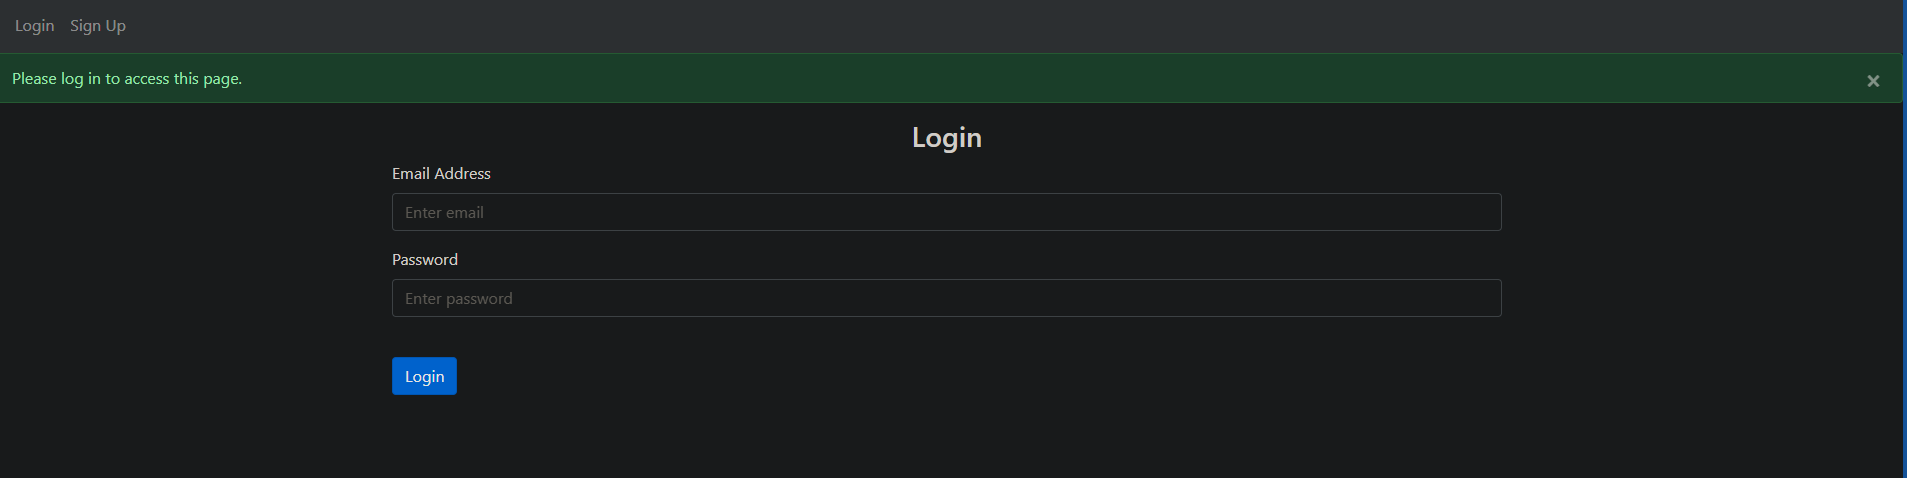
\includegraphics[width=16cm]{figs/login.png}
\caption{Página de login}
\label{fig:bookstack}
\end{center}
\end{figure}


Neste projeto foi usada como base de dados o SQLAlchemy do próprio Flask com a
seguinte estrura.
\begin{lstlisting}[language=csh, caption={Estrutura da base de dados}]
from . import db
from flask_login import UserMixin
from sqlalchemy.sql import func


class User(db.Model, UserMixin):
    id = db.Column(db.Integer, primary_key=True)
    email = db.Column(db.String(150), unique=True)
    password = db.Column(db.String(150))
\end{lstlisting}


Já no processo de autenticação os dados recebidos através do formulário da
página para serem verificados pelo seguinte código.

\begin{lstlisting}[language=csh, caption={Autenticação na página de login}]
@auth.route('/login', methods=['GET', 'POST'])
def login():
    if request.method == 'POST':
        email = request.form.get('email')
        password = request.form.get('password')

        user = User.query.filter_by(email=email).first()
        if user:
            if check_password_hash(user.password, password):
                flash('Login efetuado com sucesso!', category='success')
                login_user(user, remember=True)
                return redirect(url_for('views.home'))
            else:
                # messagem de erro opcional, o admin do sistema deve decidir se quer usar ou nao
                flash('Password incorreta', category='error') # pass incorreta
        else:
            flash('Credencias incorretas ou nao registadas', category='error') # email nao registado

    return render_template("login.html", user=current_user)
\end{lstlisting}

O \textit{email} e a hash (sha 256) da \textit{password} inseridos são verificados 
se existem na base de dados, se sim, a sessão é iniciada, caso contrário, o utilizador 
continua na página de \textit{login} e recebe (configuração de aviso de erro opcional
das linhas 13 e 16) um aviso do erro na página. \\




No caso da página de registo, poderá opcionalmente ser desativada, uma vez que 
apenas um numero mínimo
de utilizadores deverá ter acesso à funcionalidades de gestão de portas. \\

\begin{figure}[H]
\begin{center}
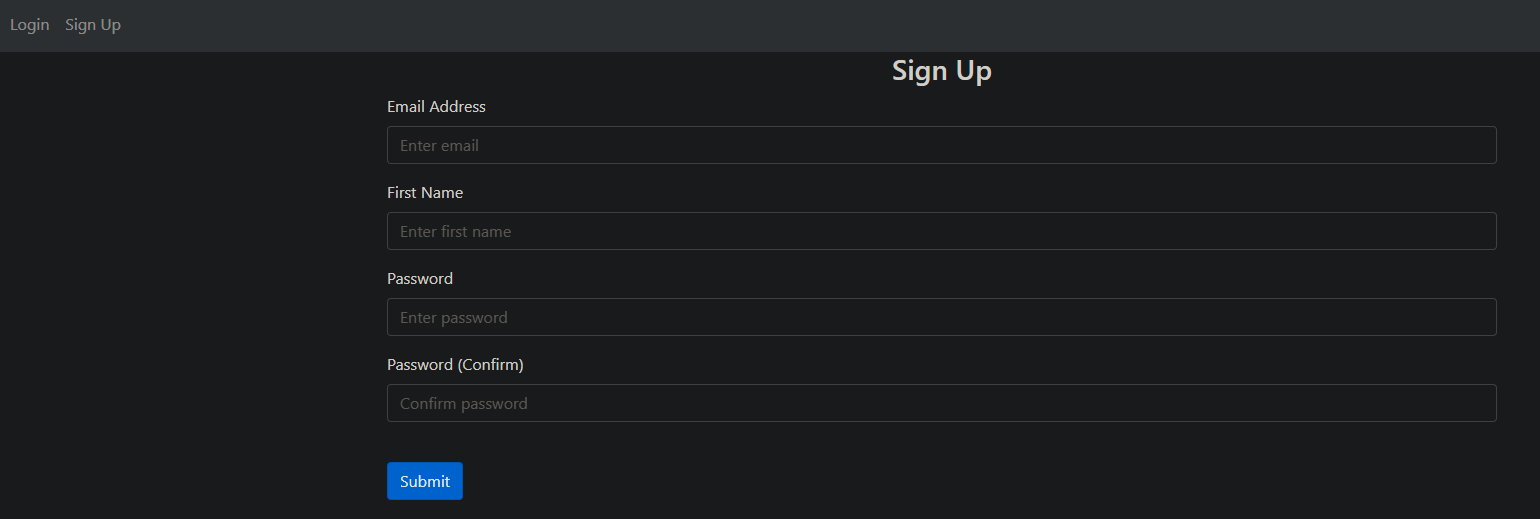
\includegraphics[width=16cm]{figs/registo.png}
\caption{Página de registo}
\label{fig:bookstack}
\end{center}
\end{figure}




\subsection{Página para fazer pedidos sobre portas}

\begin{figure}[H]
\begin{center}
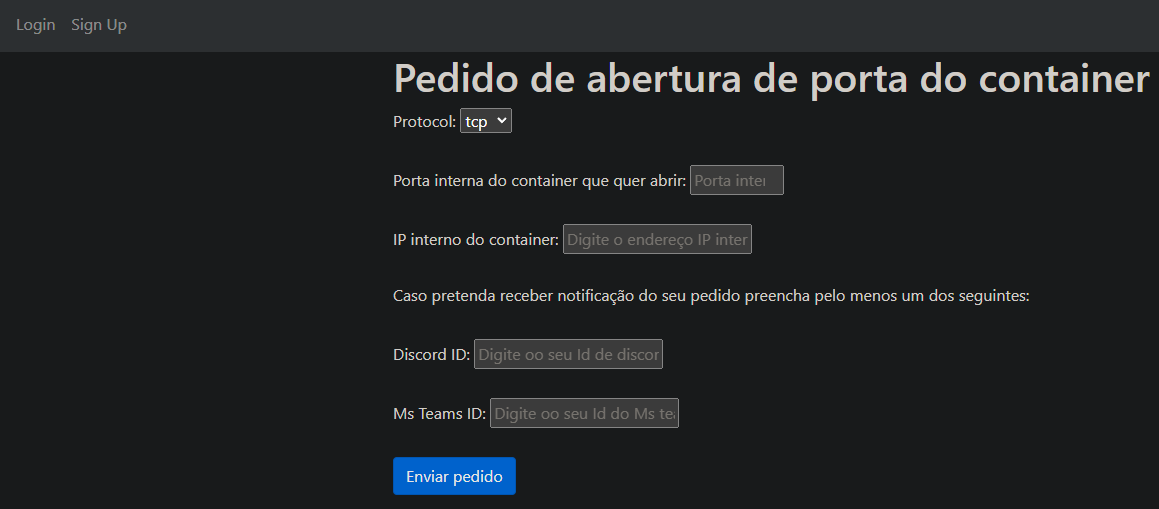
\includegraphics[width=16cm]{figs/pedido3.png}
\caption{Página de de pedidos}
\label{fig:bookstack}
\end{center}
\end{figure}

Nesta pagina é possível inserir os dados para fazer o pedido ao administrador do
sitema para abrir uma determinada porta de modo dar aos utilizazdores da rede local
conectividade ao serviço aloja no \textit{container} na porta em questão. \\

Opcionalmente, é possivel inserir o ID do Discord ou Microsoft Teams para receber
notificação sobre o pedido.

\subsection{Página para criar a ligação NAT}

\begin{figure}[H]
\begin{center}
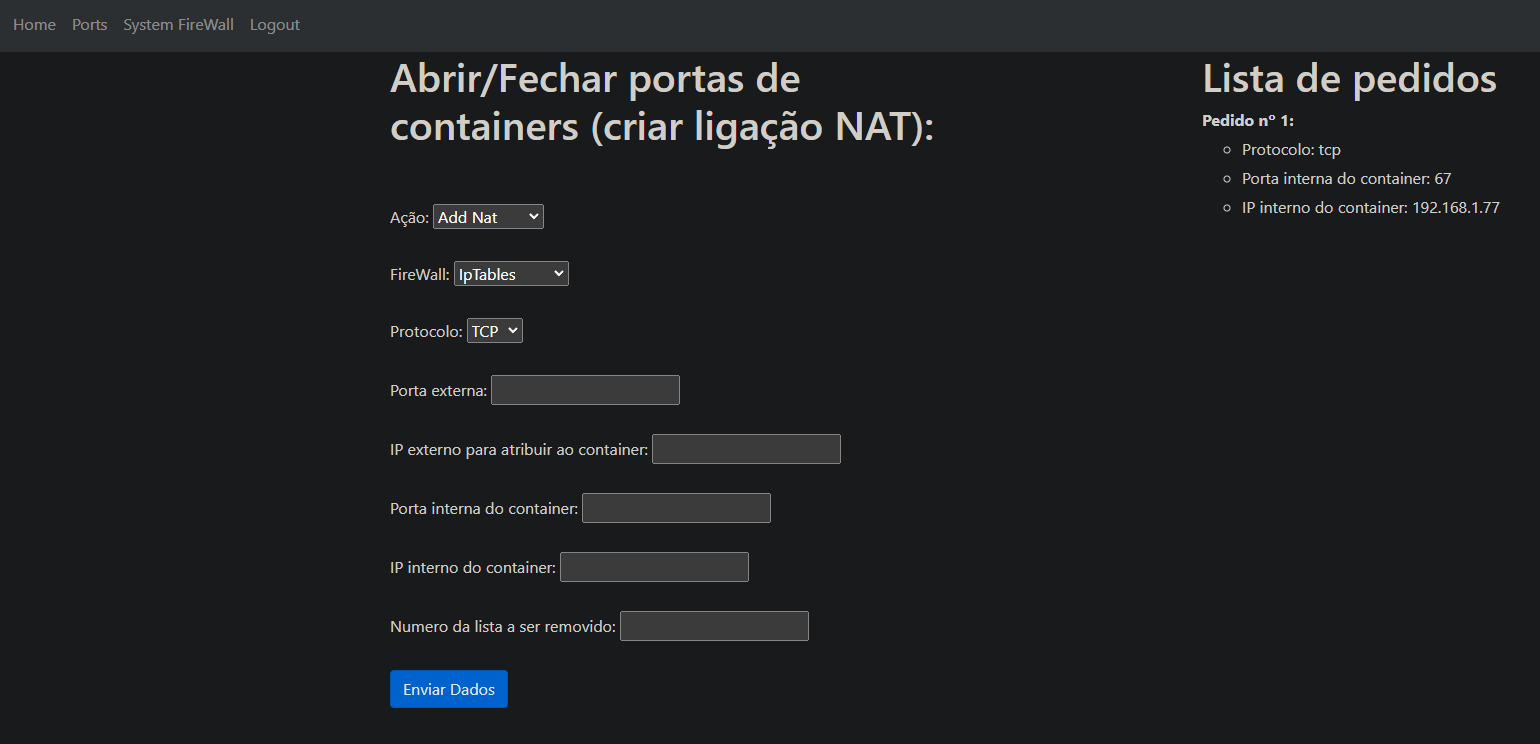
\includegraphics[width=16cm]{figs/criar nat 2.png}
\caption{Página para criar ligações NAT}
\label{fig:bookstack}
\end{center}
\end{figure}

O administrador do sistema ao inserir as suas credênciais tem acesso à página
para criar a ligação NAT. Nesta pagina é apresentado do lado direito
os pedidos pendentes, podendo associar uma porta juntamente com 
endereço IP do \textit{container} com uma porta e endereço IP exerternos. \\

O seguinte excerto de código mostra uma função em javascript onde é verificado
se todos os campos foram preenchidos e aplicada uma 
expressão regular para os campos de endreçoes IP, para garantir o formato correto.

\begin{lstlisting}[language=csh, caption={Código em javascript par verificar parâmetros da interface web}]
function validateForm() {
    const action = document.getElementById("action").value;
    const fw = document.getElementById("fw").value;
    const protocol = document.getElementById("protocol").value;
    const extPort = document.getElementById("ext_port").value;
    const extIp = document.getElementById("ext_ip").value;
    const intPort = document.getElementById("int_port").value;
    const intIp = document.getElementById("int_ip").value;

    if (!action || !fw || !protocol || !extPort || !extIp || !intPort || !intIp) {
        alert("Todos os campos devem ser preenchidos!");
        return false;
    }

    const ipPattern = /^(25[0-5]|2[0-4][0-9]|1[0-9]{2}|[1-9]?[0-9])(\.(25[0-5]|2[0-4][0-9]|1[0-9]{2}|[1-9]?[0-9])){3}$/;
    if (!ipPattern.test(intIp)) {
        alert("Por favor, insira um endereco IP valido.");
        return false;
    }

    if (!ipPattern.test(extIp)) {
        alert("Por favor, insira um endereco IP valido.");
        return false;
    }

    return true;
}
\end{lstlisting}




O seguinte excerto de código python mostra o que acontece quando os dados são enviados.
\begin{lstlisting}[language=csh, caption={Código em python da interface web}]
@views.route('/nat', methods=['GET', 'POST']) 
def nat():

    if request.method == 'POST':
        
        action = request.form.get('action')
        fw = request.form.get('fw')
        protocol= request.form.get('protocol')
        ext_port = request.form.get('ext_port')
        ext_ip = request.form.get('ext_ip')
        int_port = request.form.get('int_port')
        int_ip = request.form.get('int_ip')
        chave = request.form.get('key_to_remove')
        
        
        try:
            notificar(int(chave))
            remove_item(int(chave))
        except:
            print("Erro nao foi recebido nenhum valor para remover da lista de pedidos")


        print(action)
        print(fw)
        print(protocol)
        print(ext_port)
        print(ext_ip)
        print(int_port)
        print(int_ip)
        
        hostnat(action, fw, protocol, ext_port, ext_ip, int_ip, int_port)
        return redirect(url_for('views.nat', dicionario=pedidos , user=current_user))

    return render_template('nat.html', dicionario=pedidos , user=current_user)
\end{lstlisting}

É possivel reparar que este código recebe os dados do formulário preenchido da página HTML
para, de seguida, na linha 17 serem enviadas notificações para os utilizadores que inseriram
pelo menos um ID (Discord ou Microsoft Teams).

Na linha 18 é removido o pedido, referente aos dados preenchidos, do dicionário no qual estava guardado.

Na linha 31 é chamada a função "hostnat" do ficheiro "unisSocketConn.py" onde são passados 
os valores do formulário para serem enviados para o "Port Controller" e por sua vez execudada
a ação de acordo com esses mesmos dados.

Por fim na linha 32, a página é atualizada e juntamente com o contéuda do dicionário "pedidos".





\title*{\textbf{Página para abrir/fechar portas do sistema host}}

\begin{figure}[H]
\begin{center}
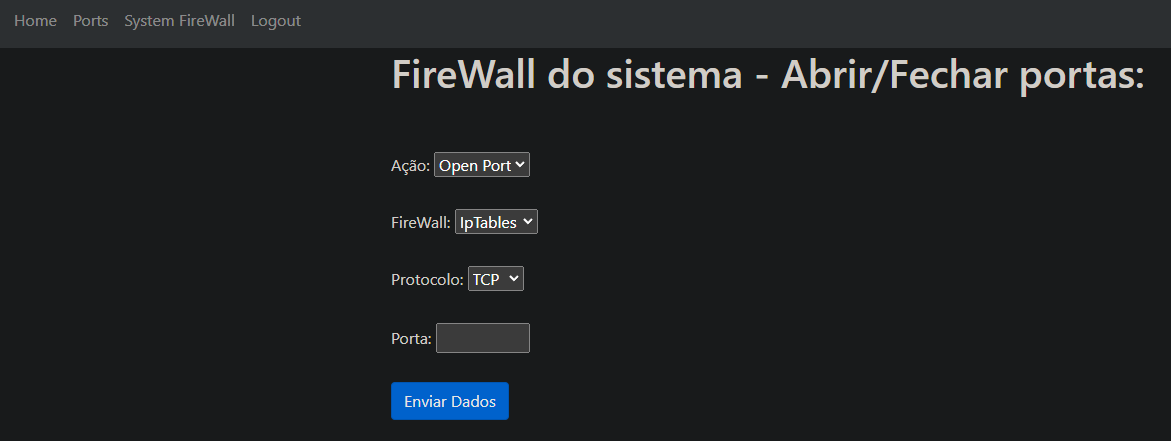
\includegraphics[width=16cm]{figs/sysfirewall.png}
\caption{Página de da firewall do sistema}
\label{fig:bookstack}
\end{center}
\end{figure}

É também possível abrir e fechar portas da \textit{firewall} (Iptables) 
do sistema \textit{host}.








%================================================================================

\section{Sistema de notificações}

Para notificar os utilizadores que fizeram pedidos para abrir uma determinada
porta podem opcionalmente receber uma notificação quando o seu pedido é aceite 
através do Discord ou Microsoft Teams.

\subsection{Discord}

Para a implemetação de enviar notificações para um utilizador no Discord,
não foi criado um "\textit{Bot}", mas sim uma conta normal, uma vez que o objetivo é apenas
enviar mensagem direta para um utilizador e não gerir um servidor.

\begin{lstlisting}[language=csh, caption={Envio de notificação via Discord}]
import os
from dotenv import load_dotenv, dotenv_values
import requests

#load from .env
load_dotenv('.env')
key: str = os.getenv('KEY')


def createDm(user_id):
    payload = {
        'recipient_id': user_id
    }
    
    header = {
        'Content-Type': 'application/json',
        'authorization': key
    }

    url = "https://discord.com/api/v9/users/@me/channels"
    
    r = requests.post(url, json=payload, headers=header)
    print(r.status_code)
    #print(r.json())

    channel_id = r.json()['id']
    
    return channel_id

def send_dm(user_id):

channel_id = createDm(user_id)

url = f"https://discord.com/api/v9/channels/{channel_id}/messages"


header = {  
    'authorization': key
}

payload = {
    'content': "O seu pedido foi conluido"
}


r = requests.post(url, data=payload, headers=header)
print(r.status_code)
\end{lstlisting}

Neste excerto de código é carregado de um ficheiro .env o token da conta, usado para
a autenticação das solicitações feitas ao longo do procedimento.

A função "createDm" (linha 10) envia uma solicitação POST apenas para criar o canal de texto
com o utilizador e enviar o ID desse mesmo canal para a função "send\_dm".

Para de seguida, a função "send\_dm" (linha 30) enviar a mensagem (solicitação POST) para 
o canal. Fazendo assim, que o utilizador receba uma mensagem direta.

Sendo assim, é apenas chamar a função "send\_dm" e passar-lhe o argumento do ID do utilizador. \\



%======================================================================================

\subsection{Microsoft Teams}

Para enviar notificações para um utilizador via Miscrosoft Teams, ao contrário do Discord,
é necessário criar um \textit{Bot} com um Framewok fornecido pela Microsoft.


\title*{\textbf{Registo do Bot no Azure}}

Para poder criar um Bot para o Microsoft Teams é necessário registar o mesmo 
no "Azure Bot" do \textit{Marketplace} do Azure.

\begin{figure}[H]
\begin{center}
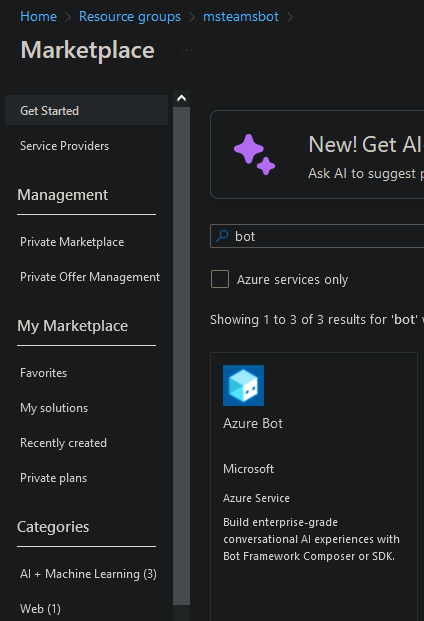
\includegraphics[width=14cm]{figs/marketplace azure bot.png}
\caption{Azure Bot do Marketplace do Azure}
\label{fig:bookstack}
\end{center}
\end{figure}

De seguida é apenas necessário preencher os parâmetros necessários de modo a obter
a seguinte configuração.

\begin{figure}[H]
\begin{center}
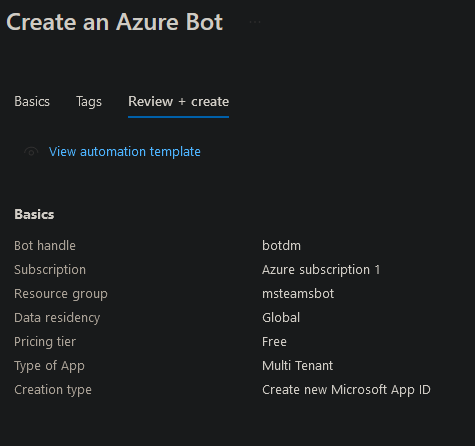
\includegraphics[width=14cm]{figs/detalhes do bot.png}
\caption{Detalhes do registo do BOT}
\label{fig:bookstack}
\end{center}
\end{figure}


\title*{\textbf{Funcionamento do código}

Para garatir o funcionamento do bot é necessário instalar as seguintes bibliotecas:
\begin{itemize}
    \item botbuilder-core
    \item botbuilder-schema
    \item botbuilder-integration-aiohttp
    \item aiohttp
\end{itemize}

O seguinte excerto de código mostra o funcionamento do envio de mensagens via Microsoft Teams.

\begin{lstlisting}[language=csh, caption={Envio de notificação via Microsoft Teams}]
from aiohttp import web
from botbuilder.core import BotFrameworkAdapter, BotFrameworkAdapterSettings, TurnContext
from botbuilder.schema import Activity, ActivityTypes, ConversationReference

import os
import asyncio

app_id = os.getenv("MICROSOFT_APP_ID", "my-app-id")
app_password = os.getenv("MICROSOFT_APP_PASSWORD", "my-app-password")
settings = BotFrameworkAdapterSettings(app_id, app_password)
adapter = BotFrameworkAdapter(settings)


conversation_references = {}

async def send_proactive_message(conversation_reference: ConversationReference, message: str):
    async def aux(turn_context: TurnContext):
        await turn_context.send_activity(Activity(type=ActivityTypes.message, text=message))

    await adapter.continue_conversation(conversation_reference, aux, app_id)

async def messages(req: web.Request) -> web.Response:
    body = await req.json()
    activity = Activity().deserialize(body)

    if activity.type == ActivityTypes.message and "Ola" in activity.text:
        # Criar a referencia da conversa
        conversation_reference = TurnContext.get_conversation_reference(activity)
        user_id = activity.from_property.id
        conversation_references[user_id] = conversation_reference

        # Enviar mensagem para o utilizador
        asyncio.create_task(send_proactive_message(conversation_reference, "Ola! o seu pedido foi concluido."))

    return web.Response(text="OK")


async def send_message_to_user(req: web.Request) -> web.Response:
data = await req.json()
user_id = data.get("user_id")
message = data.get("message")

if user_id in conversation_references:
    conversation_reference = conversation_references[user_id]
    await send_proactive_message(conversation_reference, message)
    return web.Response(text="Mensagem enviada.")
else:
    return web.Response(status=404, text="Utilizador nao encontrado.")



app = web.Application()
app.router.add_post("/api/messages", messages)
app.router.add_post("/api/send-message", send_message_to_user)

if __name__ == "__main__":
    port = int(os.environ.get('PORT', 3900))
    web.run_app(app, port=port)

\end{lstlisting}

O código apresentado deve estar a ser executado num servidor que seja acessivel pela
aplicação da interface \textit{web} para apartir desta, ser enviada uma solicitação POST
para o caminho "/api/send-message". \\

O seguinte excerto de código mostra a função que é chamada apartir da aplicação
da interface \textit{web} para enviar notificação para os utilizadores.
\begin{lstlisting}[language=csh, caption={Solicitação para enviar mensagem}]
import requests

def SendeDm(user_id):

    payload = {
        "user_id": user_id,
        "message": "O seu pedido foi conluido"
    }
    
    header = {
        'Content-Type': 'application/json'
    }

    url = "http://localhost:3900/api/send-message"
    
    r = requests.post(url, data=payload, headers=header)
    print(r.status_code)
\end{lstlisting}

Esta funcionalidae de notificações pode ser testada também com o seguinte comando.
\begin{lstlisting}[language=csh, caption={Teste de notificação via Microsoft Teams}]
    curl -X POST -H "Content-Type: application/json" -d '{"user_id": "USER_ID", "message": "conteudo da mensagem direta"}' http://localhost:3978/api/send-message
\end{lstlisting}


\section*{Sumário}

Ver o \nameref{sec:intro_summary} página \pageref{sec:intro_summary} para perceber como utilizar esta secção.






